\section{Durchführung}

    \noindent In diesem Versuch wird die Aufbau aus Abbildung(\ref{img:Versuch})

    \begin{figure}[ht]
        \centering
        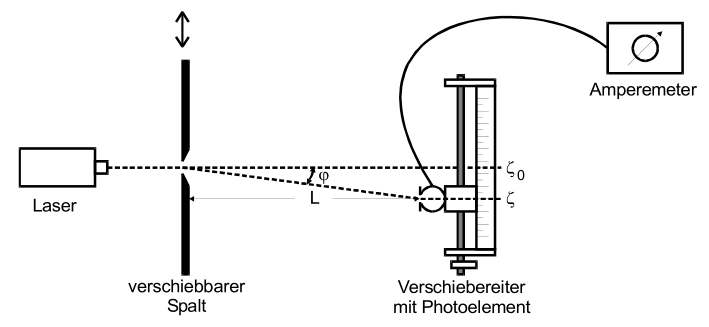
\includegraphics[width=0.5\textwidth]{latex/images/Versuch.PNG}
        \caption{Versuchsanordnung \protect \cite{V406}.}
        \label{img:Versuch}
    \end{figure}

    \noindent verwendet, jediglich der verschiebbare Spalt wird nicht genutzt. Der Laser ist ein He-Ne-Laser mit einer Wellenlänge von 
    $\SI{633}{\nano\meter}$ und leuchtet entweder auf einen Einzel- oder Doppelspalt. Etwa $\SI{140}{\centi\meter}$ hinter dem Spalt ist der 
    Detektor aus einer Photodiode auf einem Verschiebereiter aufgebaut. Das Photoelement nimmt auch im dunkeln einen Dunkelstrom
    $I_{\text{du}}$ auf, dieser wird zu Anfang des Versuch bei abgedecktem Sensor gemessen.\\

    \noindent Der gesamte Versuchsaufau wird justiert indem zunächst der Detektor auf die Mittelstellung gestellt wird, dann wird der Laser so eingestellt, 
    dass das Maximum genau auf dem Mittelpunkt des Sensors liegt. Nun wird je nach Versuch der Einzel- oder Doppelspalt so in die Vorrichtung 
    gesetzt, dass die maximale Intensität am Sensor ankommt, die Nebenmaxima sollten auf beiden Seiten ungefähr die gleiche Intensität haben.\\

    \noindent Nun werden für die beiden Teilversuche mit dem Einzel- und Doppelspalt über die $\SI{50}{\milli\meter}$ Verschiebeweg des Sensors, 
    mindestens 50 Datenpunkte aufgenommen. Der Bereich um das Maximum im Zentrum sollte dabei genauer als die Außenbereiche ausgemessen werden.


    